\documentclass{article}
\usepackage{graphicx} % Required for inserting images
\usepackage{amsmath}
\usepackage{marginnote}
\usepackage{amssymb}


\title{Projet Maths}
\author{Matthias ZDRAVKOVIC, Ameen MOHD FAIRUZ}
\date{Mai 2023}

\begin{document}

\maketitle

\section{Introduction}

Dans ce projet nous allons étudier la loi normale bidimensionnelle et essayer de la représenter graphiquement.
Nous allons essayer de trouver une équation d'ellipse d'isodensité de cette loi, et calculer la probabilité qu'un point tiré selon cette loi appartienne à cette ellipse, et proposer 
un estimateur des valeurs de $\mu$ et $\Sigma$. Puis, nous essayerons de prouver ces estimateurs en faisant une étude numerique sur python.

\section{Développements mathématiques}

\reversemarginpar\marginnote{1. a)}[0cm]

On part de la loi normale bidimensionnelle :
$$f_Z(z) = \frac{1}{2\pi \sqrt{\det \Sigma}}exp(-\frac{1}{2}{}^{t}(z-\mu)\Sigma^{-1}(z-\mu))$$
On pose
$$\Sigma = U \cdot \Lambda \cdot U^T$$
$$ \Leftrightarrow \det \Sigma = \det U \cdot \det \Lambda \cdot \det (U^T) $$
\begin{center}
$(\det U)^{2}=1$ car c'est une matrice orthogonale
\end{center}
$$\Leftrightarrow \det \Sigma =\det \Lambda$$
avec $\Sigma \in M_2(\mathbb{R})$ matrice symétrique positive définie, $U \in M_2(\mathbb{R})$ matrice orthogonale et $\Lambda \in M_2(\mathbb{R})$ matrice diagonale à coefficients positifs.\\
On pose
\[
U = \begin{pmatrix}
    \cos(\theta) & -\sin(\theta) \\
    \sin(\theta) & \cos(\theta)
\end{pmatrix}
\]
et 

\[
\Lambda = \begin{pmatrix}
    a & 0 \\
    0 & b
\end{pmatrix}
\]
avec 
$$ \Sigma^{-1} = U \cdot \Lambda^{-1} \cdot U^{-1}$$
$$\Leftrightarrow \Sigma^{-1} = \begin{pmatrix} \cos(\theta) & -\sin(\theta) \\ \sin(\theta) & \cos(\theta) \end{pmatrix} \cdot \begin{pmatrix} \frac{1}{a} & 0 \\ 0 & \frac{1}{b} \end{pmatrix} \cdot \begin{pmatrix} \cos(\theta) & -\sin(\theta) \\ \sin(\theta) & \cos(\theta) \end{pmatrix}^{-1}$$
$$\Leftrightarrow \Sigma^{-1} = \begin{pmatrix} \cos(\theta) & -\sin(\theta) \\ \sin(\theta) & \cos(\theta) \end{pmatrix} \cdot \begin{pmatrix} \frac{1}{a} & 0 \\ 0 & \frac{1}{b} \end{pmatrix} \cdot \frac{1}{\cos^{2} \theta + \sin^{2} \theta}\begin{pmatrix} \cos(\theta) & \sin(\theta) \\ -\sin(\theta) & \cos(\theta) \end{pmatrix}$$
$$\Leftrightarrow \Sigma^{-1} = \begin{pmatrix} \cos(\theta) & -\sin(\theta) \\ \sin(\theta) & \cos(\theta) \end{pmatrix} \cdot \begin{pmatrix} \frac{1}{a} & 0 \\ 0 & \frac{1}{b} \end{pmatrix} \cdot \begin{pmatrix} \cos(\theta) & \sin(\theta) \\ -\sin(\theta) & \cos(\theta) \end{pmatrix}$$
$$\Leftrightarrow \Sigma^{-1} = \begin{pmatrix} \frac{b\cos^{2} \theta + a\sin^{2} \theta}{ab} & \frac{b\sin \theta\cos \theta - a\sin \theta\cos \theta}{ab} \\ \frac{b\sin \theta\cos \theta - a\sin \theta\cos \theta}{ab} & \frac{b\sin^{2} \theta + a\sin^{2} \theta}{ab}\end{pmatrix} $$

On injecte dans la formule de $f_Z(z)$ :
$$f_Z(z) = \frac{1}{2\pi \sqrt{ab}}exp(-\frac{1}{2}\begin{pmatrix}x-\mu_1 & y-\mu_2 \end{pmatrix}\cdot\begin{pmatrix} \frac{b\cos^{2} \theta + a\sin^{2} \theta}{ab} & \frac{b\sin \theta\cos \theta - a\sin \theta\cos \theta}{ab} \\ \frac{b\sin \theta\cos \theta - a\sin \theta\cos \theta}{ab} & \frac{b\sin^{2} \theta + a\sin^{2} \theta}{ab}\end{pmatrix}\begin{pmatrix}x-\mu_1 \\ y-\mu_2 \end{pmatrix})$$
\begin{multline*}\Leftrightarrow f_Z(z) = \frac{1}{2\pi \sqrt{ab}}exp(-\frac{1}{2ab}\begin{pmatrix}x-\mu_1 & y-\mu_2 \end{pmatrix}\cdot\begin{pmatrix} b\cos^{2} \theta + a\sin^{2} \theta & b\sin \theta\cos \theta - a\sin \theta\cos \theta \\ b\sin \theta\cos \theta - a\sin \theta\cos \theta & b\sin^{2} \theta + a\sin^{2} \theta\end{pmatrix}\\\cdot \begin{pmatrix}x-\mu_1 \\ y-\mu_2 \end{pmatrix})\end{multline*}

Calculons le produit matriciel A dans l'exponentielle :

$$ A=\begin{pmatrix}x-\mu_1 & y-\mu_2 \end{pmatrix}\cdot\begin{pmatrix} b\cos^{2} \theta + a\sin^{2} \theta & b\sin \theta\cos \theta - a\sin \theta\cos \theta \\ b\sin \theta\cos \theta - a\sin \theta\cos \theta & b\sin^{2} \theta + a\sin^{2} \theta\end{pmatrix}\cdot \begin{pmatrix}x-\mu_1 \\ y-\mu_2 \end{pmatrix}$$ 
\begin{multline*} \Leftrightarrow A=((a\sin^2\theta+b\cos^2\theta)(x-\mu_1)+\cos\theta\sin\theta(b-a)(y-\mu_2))(x-\mu_1)\\+((b\sin^2\theta+a\cos^2\theta)(y-\mu_2)+\cos\theta\sin\theta(b-a)(x-\mu_1))(y-\mu_2)\end{multline*}
\begin{multline*} \Leftrightarrow A=(a\sin^2\theta+b\cos^2\theta)(x-\mu_1)^2+\cos\theta\sin\theta(b-a)(x-\mu_1)(y-\mu_2)\\+(b\sin^2\theta+a\cos^2\theta)(y-\mu_2)^2+\cos\theta\sin\theta(b-a)(x-\mu_1)(y-\mu_2)\end{multline*}
\begin{multline*} \Leftrightarrow A=(a\sin^2\theta+b\cos^2\theta)(x-\mu_1)^2+2\cos\theta\sin\theta(b-a)(x-\mu_1)(y-\mu_2)\\+(b\sin^2\theta+a\cos^2\theta)(y-\mu_2)^2\end{multline*}
\begin{multline*} \Leftrightarrow A=a\sin^2\theta(x-\mu_1)^2+b\cos^2\theta(x-\mu_1)^2+2\cos\theta\sin\theta(b-a)(x-\mu_1)(y-\mu_2)\\+b\sin^2\theta(y-\mu_2)^2+a\cos^2\theta(y-\mu_2)^2\end{multline*}
\begin{multline*} \Leftrightarrow A=a(\sin^2\theta(x-\mu_1)^2+\cos^2\theta(y-\mu_2)^2)+2\cos\theta\sin\theta(b-a)(x-\mu_1)(y-\mu_2)\\+b(\sin^2\theta(y-\mu_2)^2+\cos^2\theta(x-\mu_1)^2)\end{multline*}
\begin{multline*} \Leftrightarrow A=a((x-\mu_1)^2\sin^2\theta+(y-\mu_2)^2\cos^2\theta-2\cos\theta\sin\theta(x-\mu_1)(y-\mu_2))\\+b((y-\mu_2)^2\sin^2\theta+(x-\mu_1)^2\cos^2\theta+2\cos\theta\sin\theta(x-\mu_1)(y-\mu_2))\end{multline*}
$$ \Leftrightarrow A=a((x-\mu_1)\sin\theta-(y-\mu_2)\cos\theta)^{2}+b((x-\mu_1)\cos\theta+(y-\mu_2)\sin\theta)^{2}$$

On obtient donc :

$$ f_Z(z) = \frac{1}{2\pi \sqrt{ab}}exp(-\frac{((x-\mu_1)\sin\theta-(y-\mu_2)\cos\theta)^{2}}{2b}-\frac{((x-\mu_1)\cos\theta+(y-\mu_2)\sin\theta)^{2}}{2a})=K$$

$$\Leftrightarrow   \frac{((x-\mu_1)\sin\theta-(y-\mu_2)\cos\theta)^{2}}{2b}+\frac{((x-\mu_1)\cos\theta+(y-\mu_2)\sin\theta)^{2}}{2a}=-\ln(K2\pi\sqrt{ab})$$

$$\Leftrightarrow   \frac{((x-\mu_1)\sin\theta-(y-\mu_2)\cos\theta)^{2}}{2b\ln(\frac{1}{K2\pi\sqrt{ab}})}+\frac{((x-\mu_1)\cos\theta+(y-\mu_2)\sin\theta)^{2}}{2a\ln(\frac{1}{K2\pi\sqrt{ab}})}=1$$

Ici, le centre de l'ellipse est donné par $\mathbf{\mu} = (\mu_1, \mu_2)$, $\sqrt{2a \log(\frac{1}{2\pi K \sqrt{ab}})}$ est la demi-longueur de l'axe principal et $\sqrt{2b \log(\frac{1}{2\pi K \sqrt{ab}})}$ la demi-longueur de l'axe secondaire, $K$ est la constante de normalisation et $\theta$ est l'angle de rotation de l'ellipse.

\reversemarginpar\marginnote{1. b)}[0cm]

Pour calculer la probabilité qu'un point tiré selon la loi $Z$ appartienne à la surface interne $S_k$ délimitée par l'ellipse d'isodensité $K$, on intègre la densité de $Z$ par la surface de l'ellipse:
$$P(Z \in S_k) = \int \frac{1}{\sqrt{2\pi^2det\Sigma}}exp(-\frac{1}{2} {}^{t}(z-\mu)\Sigma^{-1}(z-\mu)) dz$$
$$\Leftrightarrow \int\int_{S_k}^{} \frac{1}{2\pi\sqrt{ab}}exp(-\frac{[(x-\mu_1)cos\theta+(y-\mu_2)sin\theta]^2}{2a}-\frac{[(x-\mu_1)sin\theta-(y-\mu_2)cos\theta]^2}{2b})dxdy$$

Pour simplifier les calculs, on fait un changement de variable:

$$\left\{\begin{matrix}x_1=\frac{(x-\mu_1)cos\theta+(y-\mu_2)sin\theta}{\sqrt{2a}}
    \\ x_2=\frac{(x-\mu_1)sin\theta-(y-\mu_2)cos\theta}{\sqrt{2a}}
    \end{matrix}\right.$$
$$\Leftrightarrow 
\left\{\begin{matrix}x=\sqrt{2a}cos\theta x_1+\sqrt{2b}sin\theta y_1 +\mu_1
\\ y=\sqrt{2a}sin\theta x_1-\sqrt{2b}cos\theta y_1 +\mu_2
\end{matrix}\right.$$
$$\Leftrightarrow 
\frac{\partial x}{\partial x_1}=\sqrt{2a}cos\theta\; ;\; \frac{\partial x}{\partial y_1}=\sqrt{2b}sin\theta$$
$$
\frac{\partial y}{\partial x_1}=\sqrt{2a}sin\theta\; ;\; \frac{\partial y}{\partial y_1}=-\sqrt{2b}cos\theta$$

En changeant $(x,y)$ à $(x_1,y_1)$, nous avons maintenant:

$$\int\int_{S_k}^{} \frac{1}{2\pi\sqrt{ab}}exp(-x_1^2-y_1^2)\left| \begin{matrix}\frac{\partial x}{\partial x_1}
    &  \frac{\partial x}{\partial y_1}
     \\\frac{\partial y}{\partial x_1}
    & \frac{\partial y}{\partial y_1}
\end{matrix} \right|dx_1dy_1$$
$$\Leftrightarrow \int\int_{S_k}^{} \frac{1}{2\pi\sqrt{ab}}exp(-x_1^2-y_1^2)\left| -\sqrt{4ab}cos^2\theta -\sqrt{4ab}sin^2\theta\right|dx_1dy_1$$
$$\Leftrightarrow \int\int_{S_k}^{} \frac{2\sqrt{ab}}{2\pi\sqrt{ab}}exp(-x_1^2-y_1^2)dx_1dy_1$$
$$\Leftrightarrow \int\int_{S_k}^{} \frac{1}{\pi}exp(-x_1^2-y_1^2)dx_1dy_1$$

Changement en base polaire: on utilise $x_1=rcos\varphi$ et $y_1=rsin\varphi$

$$\int\int_{S_k}^{} \frac{1}{\pi}exp(-r^2)rdrd\varphi$$
$$\Leftrightarrow \frac{1}{\pi}\int_{0}^{r}\int_{0}^{2\pi} re^{-r^2}d\varphi dr$$
$$\Leftrightarrow \int_{0}^{r} 2re^{-r^2} dr$$

Or, ici il faut utiliser $r=$ l'équation de l'ellipse en base $(r,\varphi)$

Pour cela, nous reprenons l'équation de l'ellipse trouvée à la question 1.a)
$$\frac{((x-\mu_1)\sin\theta-(y-\mu_2)\cos\theta)^{2}}{2b\ln(\frac{1}{K2\pi\sqrt{ab}})}+\frac{((x-\mu_1)\cos\theta+(y-\mu_2)\sin\theta)^{2}}{2a\ln(\frac{1}{K2\pi\sqrt{ab}})}=1$$
$$\Leftrightarrow \frac{x_1^2}{\ln(\frac{1}{K2\pi\sqrt{ab}})}+\frac{y_1^2}{\ln(\frac{1}{K2\pi\sqrt{ab}})}=1$$
$$\Leftrightarrow \frac{r^2}{\ln(\frac{1}{K2\pi\sqrt{ab}})}=1$$
$$\Leftrightarrow r=\sqrt{\ln(\frac{1}{K2\pi\sqrt{ab}})}$$

Nous utilisons cette équation de $r$ comme borne superieure de notre intégrale:
$$\int_{0}^{\sqrt{\ln(\frac{1}{K2\pi\sqrt{ab}})}} 2re^{-r^2} dr$$
$$\Leftrightarrow \left[ -e^{-r^2} \right]_{0}^{\sqrt{\ln(\frac{1}{K2\pi\sqrt{ab}})}}$$
$$\Leftrightarrow -e^{-\ln(\frac{1}{K2\pi\sqrt{ab}})}+e^0$$

Nous trouvons donc:

$$p=P(Z \in S_k)$$
$$\Leftrightarrow p=1-2\pi K\sqrt{ab}$$
$$$$
%\clearpage
\reversemarginpar\marginnote{2.}[0cm]
Intuitivement, on a envie de montrer que les estimateurs de $\mu$ et $\Sigma$ sont :

\[
\mu = \begin{pmatrix} \frac{\sum_{i=1}^{N}Xi}{N} \\ \frac{\sum_{i=1}^{N}Yi}{N} \end{pmatrix} \Leftrightarrow \mu = \begin{pmatrix} \bar{X} \\ \bar{Y} \end{pmatrix} = \frac{\sum_{i=1}^{N}z_i}{N}
\]


\[
\Sigma = \begin{pmatrix}\frac{1}{N-1}\sum_{i=1}^{N}(x_i-\mu_1)^{2} & \frac{1}{N-1}\sum_{i=1}^{N}(x_i-\mu_1)(y_i-\mu_2) \\\frac{1}{N-1}\sum_{i=1}^{N}(x_i-\mu_1)(y_i-\mu_2) & \frac{1}{N-1}\sum_{i=1}^{N}(y_i-\mu_2)^{2}\end{pmatrix} = \frac{1}{N-1}\sum_{i=1}^{N}(z_i-\mu)(z_i-\mu)^{T}
\]
Montrons le grâce à la fonction log-vraisemblance. Pour commencer,
on va trouver l'estimateur de $\mu$ en maximisant la fonction log-vraisemblance :

$$\mu \rightarrow \ln \mathcal{L}(\mu | z_i)$$
$$\Leftrightarrow \ln \mathcal{L}(\mu | z_i)=\ln \prod_{i=1}^{N} \frac{1}{2\pi\sqrt{|\Sigma|}}exp(-\frac{1}{2}(z_i-\mu)^{T}\Sigma^{-1}(z_i-\mu))$$
$$= \sum_{i=1}^{N} (\ln (\frac{1}{2\pi\sqrt{|\Sigma|}}exp(-\frac{1}{2}(z_i-\mu)^{T}\Sigma^{-1}(z_i-\mu))))$$
$$= \sum_{i=1}^{N} (\ln \frac{1}{2\pi\sqrt{|\Sigma|}}) -\frac{1}{2}\sum_{i=1}^{N}((z_i-\mu)^{T}\Sigma^{-1}(z_i-\mu))$$
$$= \sum_{i=1}^{N} (\ln \frac{1}{2\pi\sqrt{|\Sigma|}}) -\frac{1}{2}\sum_{i=1}^{N}(z_i^{T}\Sigma^{-1}z_i - z_i^{T}\Sigma^{-1}\mu - \mu^{T}\Sigma^{-1}z_i + \mu^{T}\Sigma^{-1}\mu)$$
$$= \sum_{i=1}^{N} (\ln \frac{1}{2\pi\sqrt{|\Sigma|}}) -\frac{1}{2}\sum_{i=1}^{N}z_i^{T}\Sigma^{-1}z_i + \frac{1}{2}\sum_{i=1}^{N}z_i^{T}\Sigma^{-1}\mu + \frac{1}{2}\sum_{i=1}^{N}\mu^{T}\Sigma^{-1}z_i - \frac{1}{2}\sum_{i=1}^{N}\mu^{T}\Sigma^{-1}\mu$$
On dérive par rapport à $\mu$ et on cherche le maximum. En sachant que pour n'importe quel vecteur v de taille 2 et matrice M de taille 2x2, on a\footnote{https://www.di.ens.fr/~fbach/courses/fall2009/formulaire.pdf}\footnote{https://en.wikipedia.org/wiki/Matrixcalculus} : 
$$\frac{\partial (v^{T}Mv)}{\partial v} = (M+M^{T})v$$
$$\frac{\partial v^{T}M}{\partial v} = M^{T}$$
On utilise ces formules pour la dérivation matricielle :

$$\frac{\partial \ln \mathcal{L}(\mu | z_i)}{\partial \mu} = \frac{1}{2}(\sum_{i=1}^{N}z_i^{T}\Sigma^{-1}+\sum_{i=1}^{N}(\Sigma^{-1}z_i)^{T}-\sum_{i=1}^{N}(\Sigma^{-1}+(\Sigma^{-1})^{T})\cdot\mu) = 0$$
$$\Leftrightarrow \sum_{i=1}^{N}(\Sigma^{-1}+(\Sigma^{-1})^{T})\cdot\mu = \sum_{i=1}^{N}z_i^{T}\Sigma^{-1}+\sum_{i=1}^{N}(z_i^{T}(\Sigma^{-1})^{T})$$
$$\Leftrightarrow \sum_{i=1}^{N}\mu = \frac{\sum_{i=1}^{N}z_i^{T}\Sigma^{-1}+\sum_{i=1}^{N}(z_i^{T}(\Sigma^{-1})^{T})}{\sum_{i=1}^{N}(\Sigma^{-1}+(\Sigma^{-1})^{T})}$$
$$\Leftrightarrow \sum_{i=1}^{N}\mu = \sum_{i=1}^{N}z_i^{T}\frac{(\sum_{i=1}^{N}\Sigma^{-1}+((\Sigma^{-1})^{T}))}{\sum_{i=1}^{N}(\Sigma^{-1}+(\Sigma^{-1})^{T})}$$
$$\Leftrightarrow N\cdot\hat{\mu} = \sum_{i=1}^{N}z_i^{T}$$
$$\Leftrightarrow \hat{\mu} = \frac{\sum_{i=1}^{N}z_i^{T}}{N}$$

Or $\frac{\sum_{i=1}^{N}z_i^{T}}{N} = \frac{\sum_{i=1}^{N}z_i}{N}$ car c'est une somme d'un vecteur colonne.
On retrouve donc bien l'estimateur de $\mu$.
On fait la même chose pour $\Sigma$ :

$$\Sigma \rightarrow \ln \mathcal{L}(\Sigma | z_i)$$
$$\Leftrightarrow \ln \mathcal{L}(\Sigma | z_i)=\ln \prod_{i=1}^{N} \frac{1}{2\pi\sqrt{|\Sigma|}}exp(-\frac{1}{2}(z_i-\mu)^{T}\Sigma^{-1}(z_i-\mu))$$
$$= \sum_{i=1}^{N} (\ln \frac{1}{2\pi\sqrt{|\Sigma|}}exp(-\frac{1}{2}(z_i-\mu)^{T}\Sigma^{-1}(z_i-\mu)))$$
$$= \sum_{i=1}^{N}\ln \frac{1}{2\pi\sqrt{|\Sigma|}} + \sum_{i=1}^{N}(-\frac{1}{2}(z_i-\mu)^{T}\Sigma^{-1}(z_i-\mu))$$

On dérive par rapport à $\Sigma$ et on cherche le maximum.

On a aussi une autre formule de dérivation Matricielle\footnote{https://www.quora.com/What-is-the-differentiation-of-the-determinant-of-a-matrix-to-the-matrix-itself-and-why} :

$$\frac{\partial \det\Sigma}{\partial \Sigma} = \det(\Sigma)(\Sigma^{-1})^{T}$$
$$\frac{\partial a^{T}\Sigma^{T}b}{\partial \Sigma} = ab^{T}$$
avec a et b pas des fonctions de $\Sigma$.

$$\frac{\partial \ln \mathcal{L}(\Sigma | z_i)}{\partial \Sigma}=\sum_{i=1}^{N}(2\pi\sqrt{\det\Sigma}\cdot\frac{\partial }{\partial \Sigma}(\frac{1}{2\pi\sqrt{\det \Sigma}}))-\frac{1}{2}\sum_{i=1}^{N}(z_i-\mu)(z_i-\mu)^{T}=0$$
$$\frac{\partial \ln \mathcal{L}(\Sigma | z_i)}{\partial \Sigma}=\sum_{i=1}^{N}(\sqrt{\det\Sigma}\cdot(-\frac{1}{2\det\Sigma \sqrt{\det \Sigma}})\cdot\det(\Sigma)(\Sigma^{-1})^{T})-\frac{1}{2}\sum_{i=1}^{N}(z_i-\mu)(z_i-\mu)^{T}=0$$
$$\frac{\partial \ln \mathcal{L}(\Sigma | z_i)}{\partial \Sigma}=-\frac{1}{2}\sum_{i=1}^{N}\cdot(\Sigma^{-1})^{T}-\frac{1}{2}\sum_{i=1}^{N}(z_i-\mu)(z_i-\mu)^{T}=0$$

Or on sait que $\Sigma$ est une matrice de rotation, donc $\Sigma^{T}=\Sigma^{-1}$.
$$\Leftrightarrow \frac{\partial \ln \mathcal{L}(\Sigma | z_i)}{\partial \Sigma}=-\frac{1}{2}\sum_{i=1}^{N}\Sigma-\frac{1}{2}\sum_{i=1}^{N}(z_i-\mu)(z_i-\mu)^{T}=0$$
$$\Leftrightarrow \sum_{i=1}^{N}\Sigma=\sum_{i=1}^{N}(z_i-\mu)(z_i-\mu)^{T}$$
$$\Leftrightarrow N\cdot\Sigma=\sum_{i=1}^{N}(z_i-\mu)(z_i-\mu)^{T}$$
$$\Leftrightarrow \hat{\Sigma}=\frac{\sum_{i=1}^{N}(z_i-\mu)(z_i-\mu)^{T}}{N}$$

\section{Étude numérique}

\reversemarginpar\marginnote{1.}[0cm]
On souhaite représenter un échantillon de points tirés selon la loi de $Z$ ainsi que les ellipses d'isodensité
associées à des probabilités p $\in [0.3;0.5;0.9]$. 
$$$$
Nous avons choisi la valeur de $\mu$ au hasard avec $np.random$, et nous avons choisi la matrice de covariance:
\[
\Sigma = \begin{pmatrix} 3 &1.5  \\ 1 &2 \end{pmatrix} 
\]
Nous avons tiré 1000 points selon la loi de $Z$, et voici le graphique obtenu avec les ellipses d'isodensité de probabilite $p$ :

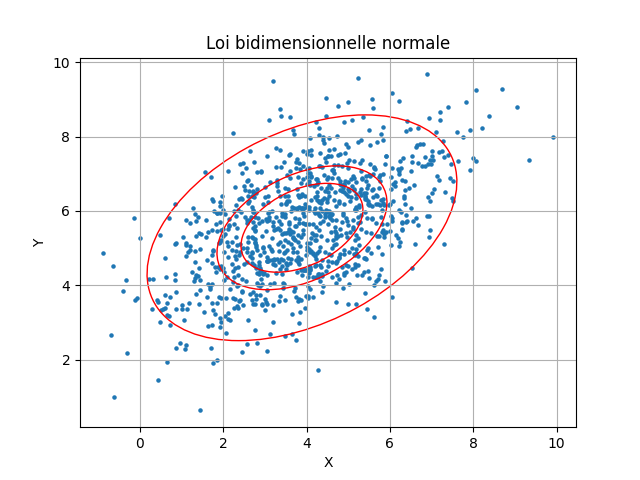
\includegraphics[width=\textwidth]{Figure_1.png}

Nous constatons que 90\% des points sont dans l'ellipse la plus grande et 50\% des points sont dans la deuxième ellipse et 30\% des points sont dans l'ellipse la plus pettite.
$$$$
\reversemarginpar\marginnote{2.}[0cm]Pour calculer la valeur des estimateurs de $\mu$ et $\Sigma$ sur des échantillons de taille variable, on prends une taille d'échantillon = 
$[1000,700,350,100]$ et nous calculons $\mu$ et $\Sigma$:

$$\hat{\mu}_1= \frac{\sum_{i=1}^{N}x_i}{N}$$
$$\hat{\mu}_2 = \frac{\sum_{i=1}^{N}y_i}{N}$$
$$\hat{\Sigma}=\frac{\sum_{i=1}^{N}(z_i-\mu)(z_i-\mu)^{T}}{N} ; z_i = (x_i,y_i)$$

Avec ces formules, nous calculons notre estimateur pour les differents tailles d'échantillon et nous tracons ces ellipses avec les probabilités $p$:

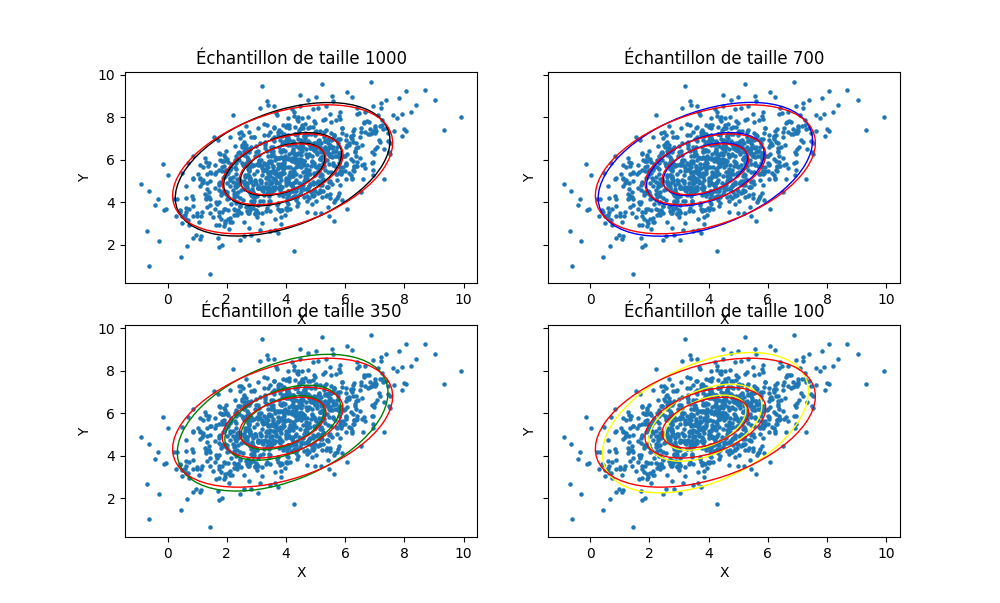
\includegraphics[width=\textwidth]{Figure_2.png}
En rouge: la vraie ellipse, En noir, bleu, vert, jaune: les ellipses formées avec les estimateurs.

Nous constatons que plus la taille de l'échantillon est grande, plus c'est précis. Donc, les estimateurs $\hat{\mu}$ et $\hat{\Sigma}$ convergent vers $\mu$ et $\Sigma$, quand la taille de l'échantillon augmente.

\section{Conclusion}
Tout au long de ce projet nous avons pu découvrir les différentes propriétés de la loi normale bidimensionnelle et nous avons pu les vérifier avec les calculs et l'étude numérique.
Nous avons pu voir que les estimateurs convergent vers les vrais paramètres de la loi normale bidimensionnelle quand la taille de l'échantillon augmente.


\end{document}

